Following test cases show the effect of defeaturing on the quality of the midsurface. Size threshold used here is certain percentage of the summation of face-areas of all the faces in the original CAD model.

\begin{enumerate}
\item Threshold (D) 3\% of the total part size


\begin{tabular}[h]{@{} p{0.12\linewidth}  p{0.28\linewidth} p{0.28\linewidth} p{0.28\linewidth}@{}}
\toprule
 & Model & Midsurface & Explanation \\
 \midrule
 
Original input &
\raisebox{-0.8\height}{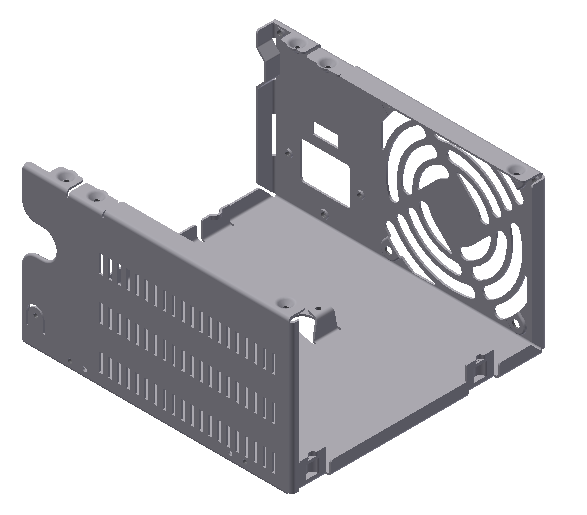
\includegraphics[width=0.8\linewidth]{..//Common/images/defeatresult_perc3_origpart}} &
\raisebox{-0.8\height}{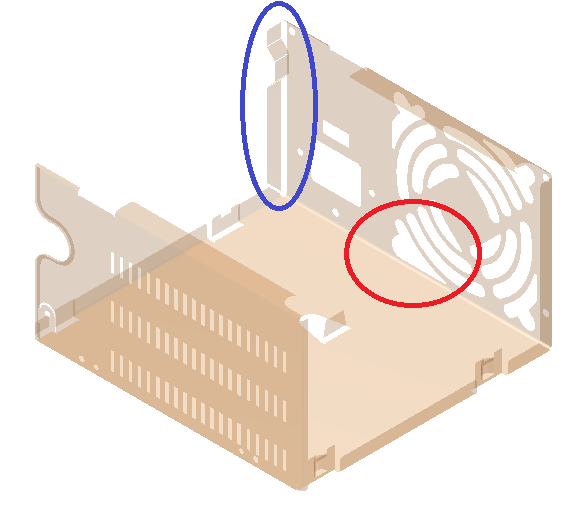
\includegraphics[width=0.8\linewidth]{..//Common/images/defeatresult_perc3_origmids}} &
Gaps in the midsurface. Two of the gaps are marked (blue and red).\\

Removing sheet metal features less than threshold &
\raisebox{-0.8\height}{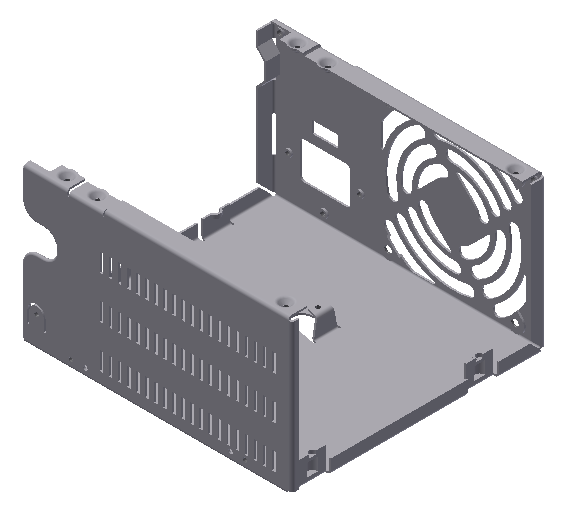
\includegraphics[width=0.8\linewidth]{..//Common/images/defeatresult_perc3_ph1part}} &
\raisebox{-0.8\height}{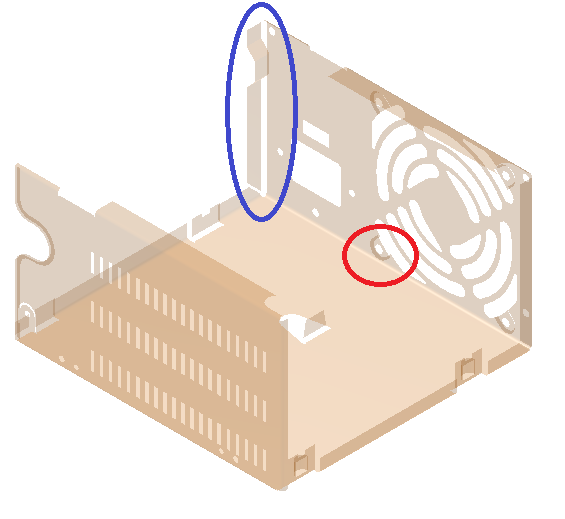
\includegraphics[width=0.8\linewidth]{..//Common/images/defeatresult_perc3_ph1mids}} &
Although the number of gaps have reduced (the red gap is filled), but the gaps between the surface patches (blue gap) is still seen. \\

Removing generic CAD features less than threshold  &
\raisebox{-0.8\height}{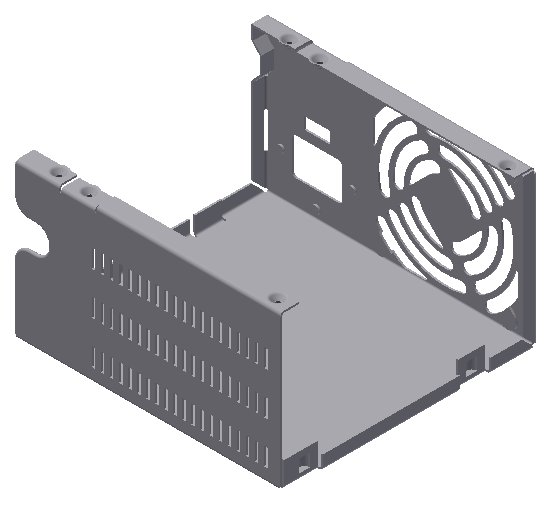
\includegraphics[width=0.8\linewidth]{..//Common/images/defeatresult_perc3_ph2part}} &
\raisebox{-0.8\height}{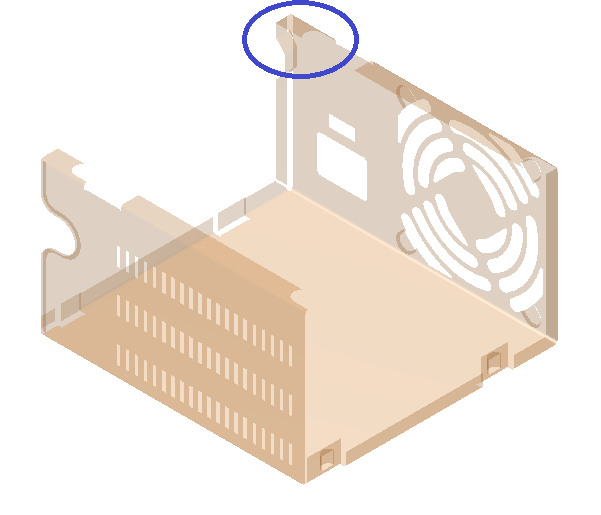
\includegraphics[width=0.8\linewidth]{..//Common/images/defeatresult_perc3_ph2mids}} &
Some of the gaps (blue gap top portion) are filled and the output is a bit better-connected midsurface. \\

\bottomrule
\end{tabular}

Effectiveness of Smarf with 3\% threshold by Eqn. \ref{eqn:defeaturing:effectiveness} is:

\begin{minipage}[c]{0.6\linewidth}
\begin{tabular}[h]{@{} p{0.22\linewidth} p{0.18\linewidth} p{0.21\linewidth} p{0.2\linewidth} @{}}\toprule
\textbf{Qty} & \textbf{Input} & \textbf{Phase I} & \textbf{Output}\\  \midrule
Faces  & 1434 & 610 & 327\\
Suppressed  &  & 60 & 30\\
\bottomrule
\end{tabular}
\end{minipage}
\begin{minipage}[c]{0.38\linewidth}
$pR = (1 - \frac{697}{833}) \times 100 = 16\%$
\end{minipage}


\item Threshold (D) 5\% of the total part size


\begin{tabular}[h]{@{} p{0.12\linewidth}  p{0.28\linewidth} p{0.28\linewidth} p{0.28\linewidth}@{}}
\toprule
 & Model & Midsurface & Explanation \\
 \midrule
 
Original input&
\raisebox{-0.8\height}{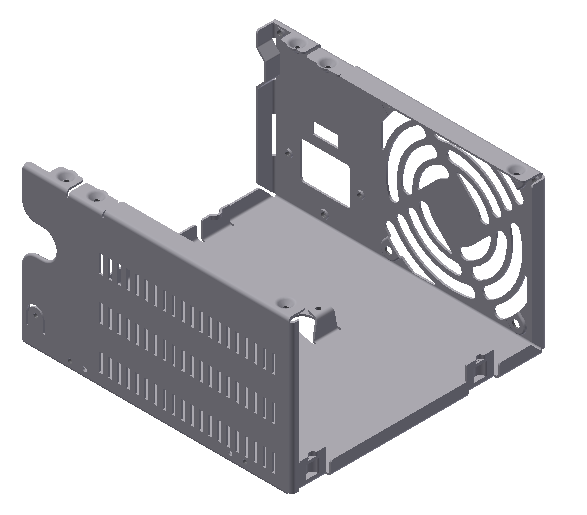
\includegraphics[width=0.8\linewidth]{..//Common/images/defeatresult_perc5_origpart}} &
\raisebox{-0.8\height}{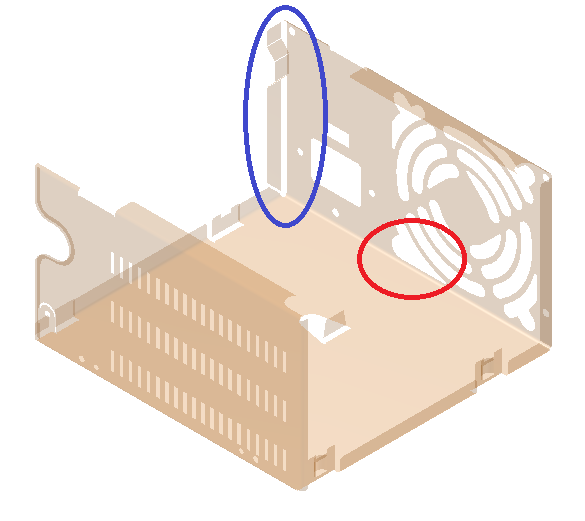
\includegraphics[width=0.8\linewidth]{..//Common/images/defeatresult_perc5_origmids}} &
Gaps in the midsurface. Two of the gaps are marked (blue and red).\\

Removing sheet metal features less than threshold &
\raisebox{-0.8\height}{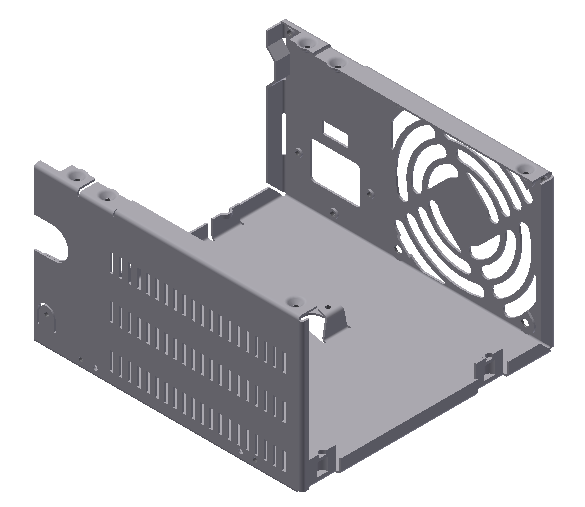
\includegraphics[width=0.8\linewidth]{..//Common/images/defeatresult_perc5_ph1part}} &
\raisebox{-0.8\height}{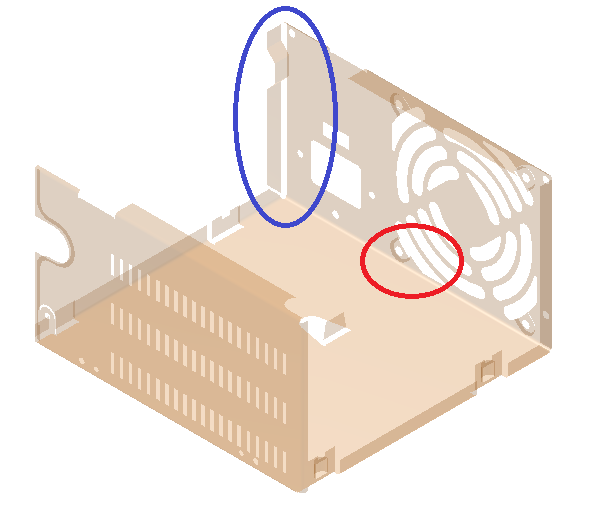
\includegraphics[width=0.8\linewidth]{..//Common/images/defeatresult_perc5_ph1mids}} &
Although the number of missing gaps in the midsurface has reduced (red gap is filled), but the gaps between the surface patches (blue gap) is still seen.\\

Removing generic CAD features less than threshold  &
\raisebox{-0.8\height}{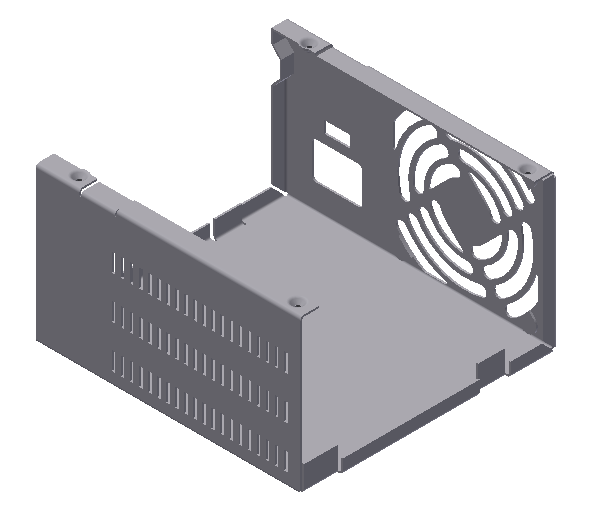
\includegraphics[width=0.8\linewidth]{..//Common/images/defeatresult_perc5_ph2part}} &
\raisebox{-0.8\height}{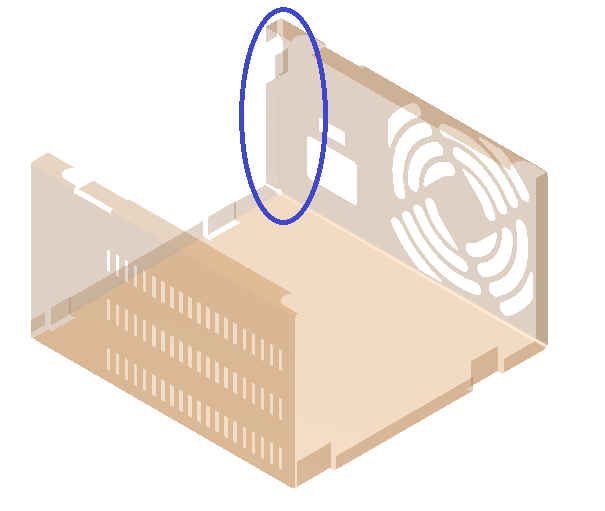
\includegraphics[width=0.8\linewidth]{..//Common/images/defeatresult_perc5_ph2mids}} &
Most of the gaps (blue gap full) are filled and the output is a better-connected midsurface. It retains all the necessary features adequately ``representing''  the gross shape. \\

\bottomrule
\end{tabular}

Effectiveness of Smarf with 5\% threshold by Eqn. \ref{eqn:defeaturing:effectiveness} is:

\begin{minipage}[c]{0.6\linewidth}
\begin{tabular}[h]{@{} p{0.22\linewidth} p{0.18\linewidth} p{0.21\linewidth} p{0.2\linewidth} @{}}\toprule
\textbf{Qty} & \textbf{Input} & \textbf{Phase I} & \textbf{Output}\\  \midrule
Faces  & 833 & 772 & 617\\
Suppressed  &  &7 & 40\\
\bottomrule
\end{tabular}
\end{minipage}
\begin{minipage}[c]{0.38\linewidth}
$pR = (1 - \frac{697}{833}) \times 100 = 26\%$
\end{minipage}

\item Threshold (D) 10\% of the total part size


\begin{tabular}[h]{@{} p{0.12\linewidth}  p{0.28\linewidth} p{0.28\linewidth} p{0.28\linewidth}@{}}
\toprule
 & Model & Midsurface & Explanation \\
 \midrule
 
Original input  &
\raisebox{-0.8\height}{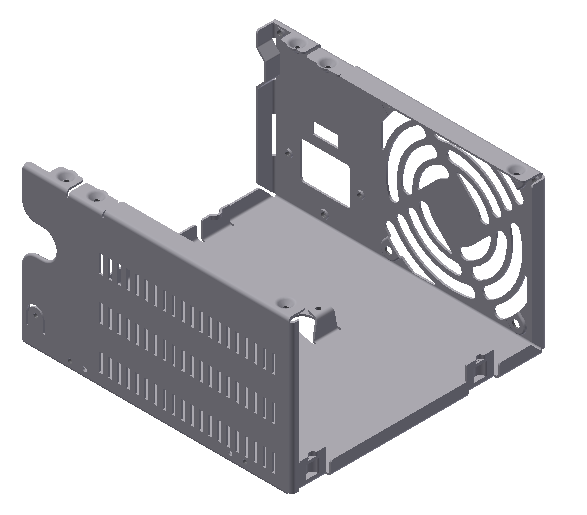
\includegraphics[width=0.8\linewidth]{..//Common/images/defeatresult_perc10_origpart}} &
\raisebox{-0.8\height}{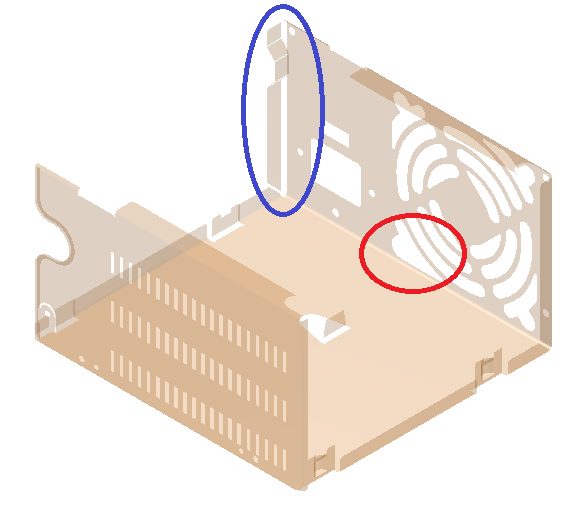
\includegraphics[width=0.8\linewidth]{..//Common/images/defeatresult_perc10_origmids}} &
Gaps in the midsurface. Two of the gaps are marked (blue and red).\\

Removing sheet metal features less than threshold &
\raisebox{-0.8\height}{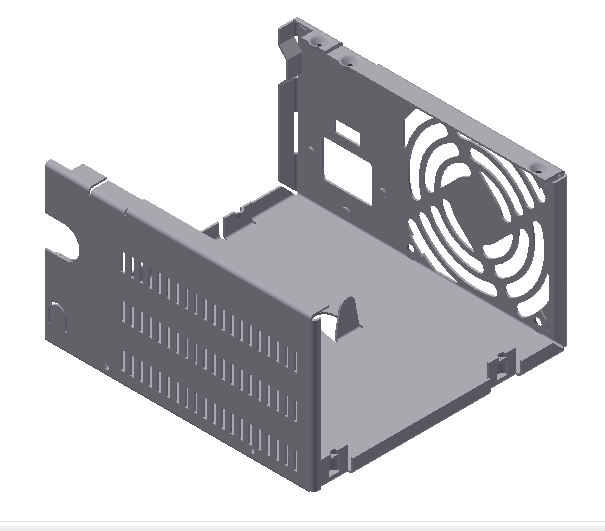
\includegraphics[width=0.8\linewidth]{..//Common/images/defeatresult_perc10_ph1part}} &
\raisebox{-0.8\height}{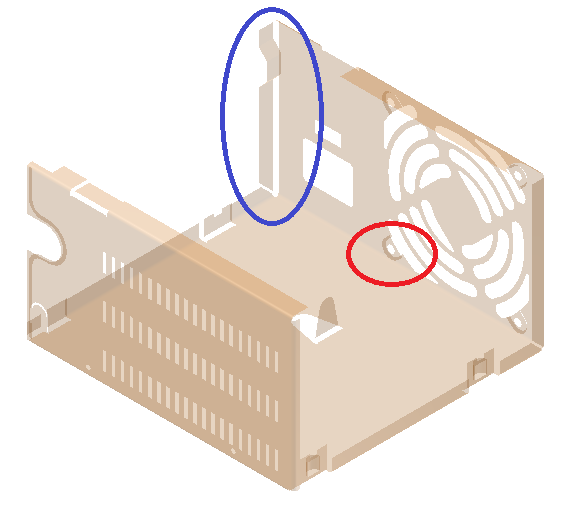
\includegraphics[width=0.8\linewidth]{..//Common/images/defeatresult_perc10_ph1mids}} &
Although the number of missing gaps in the midsurface has reduced (red gap is filled), but the gaps between the surface patches (blue gap) is still seen. \\

Removing generic CAD features less than threshold  &
\raisebox{-0.8\height}{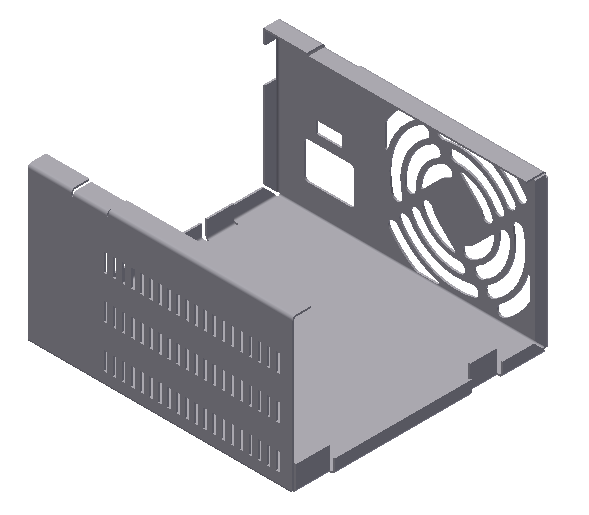
\includegraphics[width=0.8\linewidth]{..//Common/images/defeatresult_perc10_ph2part}} &
\raisebox{-0.8\height}{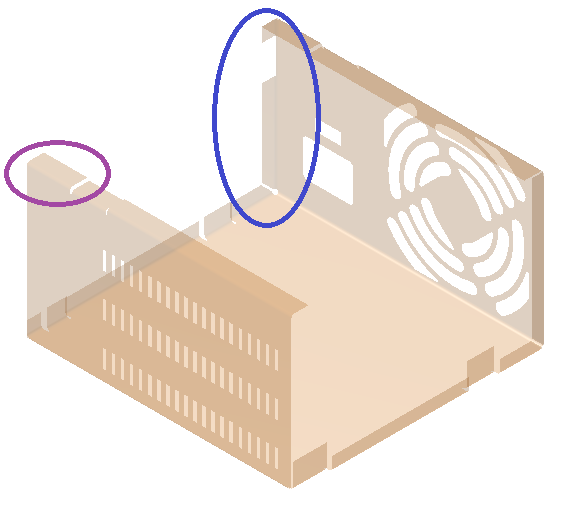
\includegraphics[width=0.8\linewidth]{..//Common/images/defeatresult_perc10_ph2mids}} &
Most of the gaps (blue gap full) are filled. Removal of purple feature could be the domain decision. It retains all the necessary features adequately ``representing''  the gross shape. \\

\bottomrule
\end{tabular}

Effectiveness of Smarf with 10\% threshold by Eqn. \ref{eqn:defeaturing:effectiveness} is:

\begin{minipage}[c]{0.6\linewidth}
\begin{tabular}[h]{@{} p{0.22\linewidth} p{0.18\linewidth} p{0.21\linewidth} p{0.2\linewidth} @{}}\toprule
\textbf{Qty} & \textbf{Input} & \textbf{Phase I} & \textbf{Output}\\  \midrule
Faces  & 833 & 715 & 522\\
Suppressed  &  &17 & 48\\
\bottomrule
\end{tabular}
\end{minipage}
\begin{minipage}[c]{0.38\linewidth}
$pR = (1 - \frac{522}{833}) \times 100 = 37\%$
\end{minipage}
\end{enumerate}

The choice of threshold can be set to such a value where midsurface output is well-connected. In the test-cases shown above 10\% appears to be the appropriate value. Increasing the threshold to still higher value results in a well-connected midsurface but it loses the shape characteristics which need to be maintained.
